\documentclass[aspectratio=43, 10pt]{beamer}
\usepackage{tutorialSlide}
\usepackage{graphicx}               % Necessary to use \scalebox
\usepackage[absolute,overlay]{textpos}

\newcommand{\curl}{{\textbf{curl}}}


\mode<presentation> {
\usetheme{AnnArbor}
\usecolortheme{dolphin}

% Configure and Customize the theme
%\setbeamertemplate{theorems}[numbered]
\setbeamercolor{alerted text}{fg=red}
% Change color scheme for blocks
\setbeamercolor*{block title example}{fg = ao(english), bg= antiquewhite}
\setbeamercolor*{block title}{fg = pigment, bg= blue!5}
\setbeamercolor*{block title alerted}{fg = red, bg= red!5}
}

\makeatletter
\newcommand\mysphere{%
  \parbox[t]{8pt}{\raisebox{0.2pt}{\beamer@usesphere{item projected}{bigsphere}}}}
\makeatother




%***************************************************************************
%***************************************************************************
\begin{document}
\title{Optimization on Stiefel Sets by Linear Search}
\subtitle{A brief introduction to a typical gradient-based algorithm}
\author{Weijia Zheng 
\thanks{I mainly take reference to: "A feasible method for optimization with orthogonality constraints" by Z. Wen, and W. Yin. 2010; and "Notes on Optimization on Stiefel Manifold" by H. D. Tagare, 2011. The latter is the most accessible document I've found about this topic.}
}

\institute[IE@CUHK] % Your institution as it will appear on the bottom of every slide, may be shorthand to save space
{
\textit{Department of Information Engineering} \\ % Your institution for the title page
\textit{The Chinese University of Hong Kong} \\
\medskip
wjzheng@link.cuhk.edu.hk % Your email address
}
\date{Sept. 27, 2024}

\setcounter{framenumber}{-1}
\frame{\titlepage}
%***************************************************************************
%***************************************************************************




\begin{frame}
\frametitle{Overview} % Table of contents slide, comment this block out to remove it
\tableofcontents % Throughout your presentation, if you choose to use \section{} and \subsection{} commands, these will automatically be printed on this slide as an overview of your presentation
\end{frame}



\AtBeginSection[]
  {
     \begin{frame}<beamer>
     \frametitle{Overview}
     \tableofcontents[currentsection]
     \end{frame}
  }
  

\section{Introduction}
  \begin{frame}[t]{Stiefel manifold}
    \vspace{-0.5cm}
    \begin{block}{Optimization on Stiefel sets}
        People aimed to develop a procedure to tackle this (non-convex for sure) optimization problem. 
        $$\min_{X_k \in \mathbb{R}^{n \times p}} F(X_1,X_2,...,X_K) ~~~~~ \text{subject to   } X_k^T X_k = I_p$$
    \end{block}

    \pause 
    \vspace{-0.1cm}
    \begin{block}{Definition of Stiefel manifold}
        Stiefel manifold, or sometimes called Stiefel set, is a set of semi-orthogonal matrices of size $n \times p$, denoted by 
        $$\mathcal{V}_p(\mathbb{R}^n) \triangleq \{ X \in \mathbb{R}^{n \times p} | X^T X = I_p\},$$
        where $I_p$ is the identity matrix of size $p \times p$.
    \end{block}
    % \vfill
    
    \pause 
    We have nothing to do with the formal definition(s) of manifold, and it suffices to just consider the above thing as a special set. However, it is good to regard a "manifold" as \textcolor{red}{a space that locally resembles Euclidean space near each point.}\footnote{Copied from the first sentence of "Manifold" Wiki-page.}
    
  \end{frame}

   \begin{frame}[t]{Why do we care about it? -- For useful applications.}
   \vspace{-0.4cm}
        \begin{block}{Low-rank nearest correlation estimation}
        Let $C \in \mathbb{S}^n$ be a given be a given symmetric matrix and $H \geq 0 $ be a nonnegative (weight) matrix. The low-rank nearest correlation estimation problem is given by 
        $$\min_{Q \in \mathbb{S}_{+}^n} \| H \odot (Q - C)\|_F^2,~~~~~\text{ subject to  } Q_{ii}=1,~ \forall i\in [n]; ~~\text{rank}(Q) \leq r,$$
        where $\mathbb{S}_{+}^n$ denotes the set of $n \times n$ positive semi-definite matrices. 
      \end{block}

      \vspace{-0.2em}
      The problem tries to find a correlation matrix\footnote{Correlation matrix should be PSD.} (which is $Q$) from an estimate $C$. $C$ may not be PSD, since it's usually a noisy estimate. 

      The rank constraint makes the problem not convex. 
      
      \pause
      \vspace{-0.45em}
      \begin{block}{Reformulation of the above}
          One can express the rank constraints explicitly as $Q = U^T U$ with $U = [U_1,..., U_n] \in \mathbb{R}^{r \times n}$ with $\|U_i\|_2=1,~~ \forall i \in [n].$ And we have 
          \small
          $$\min_{Q \in \mathbb{S}_{+}^n} \| H \odot (U^T U - C)\|_F^2,~~\text{ subject to  } \| U_i \|_2=1,~ \forall i\in [n] \iff U_i \in \mathcal{V}_1(\mathbb{R}^r) ~\forall i\in [n]$$
      \end{block}
  \end{frame}

% \section{Structures of Stiefel Sets}
  \begin{frame}[t]{Gradient descent?}
    \vspace{-0.8em}
     Let's ease ourselve with the (easier, though still hard) problem of $$\min_{X \in \mathbb{R}^{n \times p}} F(X) ~~~~~ \text{subject to   } X^T X = I_p \iff X \in \mathcal{V}_{p}(\mathbb{R}^n).$$

      \vspace{-0.5cm}
      \begin{block}{General gradient-based methods in Euclidean spaces}
          We usually use this iteration to reach a minimizer: 
          $$X_{t+1} \gets X_t - \gamma_t \nabla F(X_t)$$
      \end{block}

     \pause 
     \vspace{0.2cm}
     Difficulties come with the feasible set $\mathcal{V}_p(\mathbb{R}^n)$: 
     \begin{itemize}
         \item Non-convexity: $\mathcal{V}_{p}(\mathbb{R}^n)$ is not convex, since $\pm I_{n,p} \in \mathcal{V}_{p}(\mathbb{R}^n)$, but $0 \notin \mathcal{V}_{p}(\mathbb{R}^n).$
         \item (In)feasibility: hard to stay inside the constraint set: $\mathcal{V}_{p}(\mathbb{R}^n)$. 
     \end{itemize}

     Hopefully, we want to adapt such successful way in Euclidean spaces into our new $\mathcal{V}_p(\mathbb{R}^n)$, after some modification if needed. 

     \vspace{0.1cm}
     \textcolor{red}{And, we are not aiming to find a global-minimizer-approaching algorithm, because doing so on a manifold $\mathcal{M}$ is really hard.} Instead, what we are trying to obtain is an algorithm to generate a decreasing sequence of feasible $X_t$'s.
  \end{frame}

  \begin{frame}[t]{Tangent space of an $X\in \mathcal{M}(=\mathcal{V}_p(\mathbb{R}^n))$}
    \vspace{-0.8em}
     \begin{columns}
            % Column 2    
            \begin{column}{0.45\textwidth}
                \begin{figure}
                % \centering
                    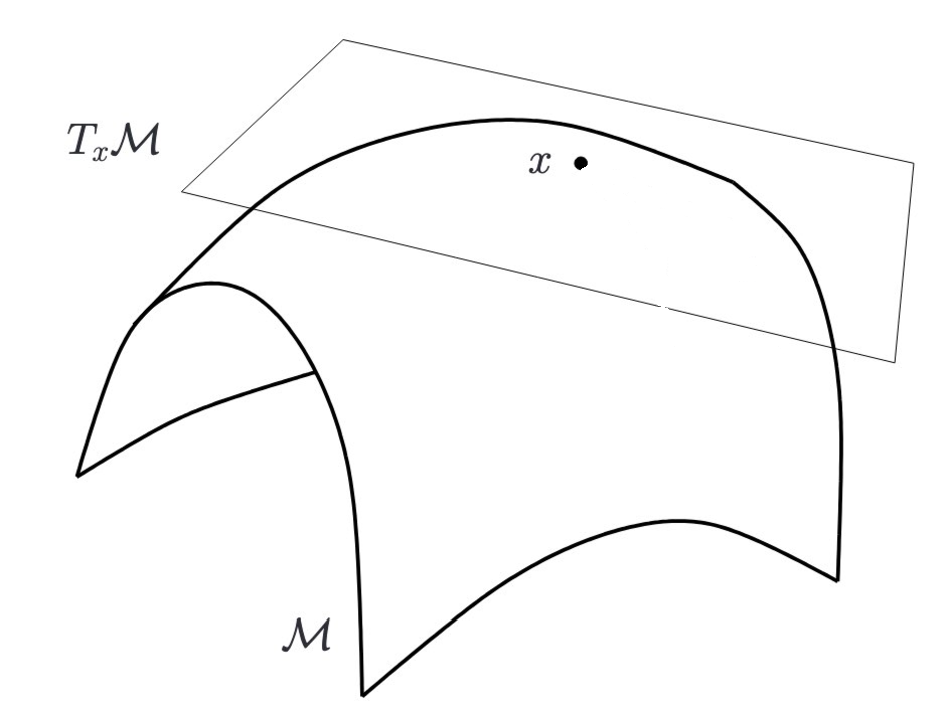
\includegraphics[width=0.9\textwidth]{figures/retraction.pdf}
                    % \caption{A figure that is next to a certain explanation.}
                \end{figure}
            \end{column}

            \begin{column}{0.5\textwidth}
               \begin{block}{Tangent space of $X \in \mathcal{M}$}
                    The tangent space (of $X$) is a "bridge" connecting the ambient $\mathbb{R}^{n \times p}$ and $\mathcal{M}$.
                    
                    Before taking a step from current $X=X_t$ towards some $X_{t+1}$, we first want to find the deepest decreasing direction at the tangent plane of $X_t$.\footnote{By the informal definition of manifold.} 

               \end{block}
            \end{column}
        \end{columns}

    \pause 
    \vspace{0.9em}
    Pick any $X \in \mathcal{V}_p(\mathbb{R}^n),$ the tangent space of $X$ is denoted as $T_X (\mathcal{V}_p(\mathbb{R}^n))$. Our next goal is to investigate the (directional) derivative starting from $X$ towards the direction $Z \in T_X (\mathcal{V}_p(\mathbb{R}^n))$. Before that, we recall the usual case for $Z \in \mathbb{R}^{n \times p}$: 
    \begin{block}{Directional derivative of $F$ at $X\in \mathcal{M}$ towards direction $Z \in \mathbb{R}^{n \times p}$}
        $$\mathcal{D}F_X[Z] \triangleq \lim_{t \to 0^+}\frac{F(X+tZ) - F(X)}{t} = \langle \mathcal{D}F_X \cdot Z \rangle_E$$
    \end{block}
  \end{frame}

\section{Representation of gradient on $T_X(\mathcal{V}_p(\mathbb{R}^n))$}
  \begin{frame}[t]{Characterising $T_X(\mathcal{V}_p(\mathbb{R}^n))$}
    \vspace{-0.8em}
    For any $X \in \mathcal{V}_p(\mathbb{R}^n)$, we know $X=[x_1, ..., x_p]$ is made up of $p$ orthonormal columns. Pick another $n-p$ new orthonormal vectors: $v_{1},...,v_{n-p}$ such that $\{x_1,...,x_p, v_1,...,v_{n-p}\}$ is a basis of $\mathbb{R}^n$. Define $X_\perp \triangleq [v_1,...,v_{n-p}] \in \mathbb{R}^{n \times (n-p)}$. 
    \begin{lemma}
        $Z = XA + X_{\perp} B \in T_X (\mathcal{V}_p(\mathbb{R}^n))$, if and only if $A = -A^T$, aka, $A$ is a skew-symmetric matrix.  
    \end{lemma}

    Side note: $0 \in T_X (\mathcal{V}_p(\mathbb{R}^n))$. The tangent space $T_X (\mathcal{V}_p(\mathbb{R}^n))$ takes $X$ as  origin. 

    \vspace{-0.3em}
        \begin{figure}
            \centering
                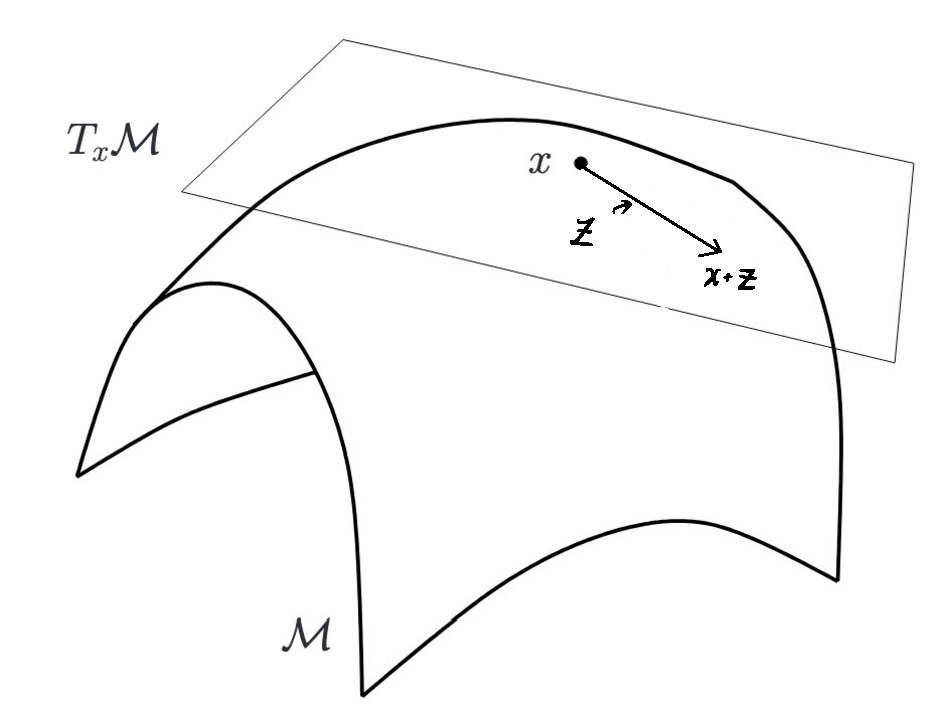
\includegraphics[width=0.45\textwidth]{figures/xorigin.pdf}
                % \caption{A figure that is next to a certain explanation.}
        \end{figure}
  \end{frame}

  \begin{frame}[t]{Inner product representation of directional derivative}
  \vspace{-0.37cm}
  In previous slides, we stated that fix any $X\in \mathcal{V}_p (\mathbb{R}^n)$, for any $Z \in \mathbb{R}^{n \times p}$ (whatever direction), 
  $$\mathcal{D}F_X[Z] = \sum_{i,j}\frac{\partial F}{\partial X_{i,j}} Z_{i,j}
  = \textbf{tr}(G^T Z) = \langle G \cdot Z \rangle_E \in \mathbb{R},$$ 
  where $G = [\frac{\partial F}{\partial X_{i,j}}] \in \mathbb{R}^{n \times p}$. \textcolor{blue}{We always use $G$ to denote the usual (Euclidean) gradient of $F$ at $X$.}

  \pause
  \vspace{-0.1cm}
  \begin{block}{Inner product representation}
      Fix any $X \in \mathcal{V}_p (\mathbb{R}^n)$, we say $G$ represents\footnote{Because $\mathcal{D}F_X[Z] = \langle G \cdot Z \rangle_E$.}  the (linear) operator $\mathcal{D}F_X: \underbrace{\mathbb{R}^{n \times p}}_{Z \in } \to \mathbb{R}$ -- which is the directional derivative -- under Euclidean standard inner product $\langle \cdot \rangle_E$.
  \end{block}

  \pause
  We then restrict $Z \in T_X \subset \mathbb{R}^{n \times p}$. Because we only move inside the $T_X$. 
  %
  We want to find (1) a matrix $W$, and (2) an inner product $\langle \cdot \rangle_C$, such that $W$ represents $\mathcal{D}F_X|_{T_X}: T_X \to \mathbb{R}$ under that inner product. Aka, $\forall Z \in T_X$, $$\mathcal{D}F_X[Z] = \langle W \cdot Z \rangle_C$$
  
  \end{frame}

  \begin{frame}{}
      \vspace{-0.1cm}
      \begin{theorem}[Representation of gradient only wrt directions in tangent space.]
      Pick any $X \in \mathcal{M} = \mathcal{V}_p (\mathbb{R}^n)$.
      Analog to $G$ represents the action of $\mathcal{D}F_X$ on $\mathbb{R}^{n \times p}$ under the standard matrix inner product $\langle \cdot \rangle_E$; 
      
      $W$, with $W \triangleq (GX^T-XG^T)X$, represents the action of $\mathcal{D}F_X$ on $T_X$ under another inner product $\langle \cdot \rangle_C$ defined as $\langle Q \cdot H \rangle_C \triangleq \textbf{tr}(Q^T (I-\frac{1}{2}XX^T)H).$ 
  \end{theorem}
     \vspace{-0.2cm}
     \pause 
  \begin{proof}
      Write $G=XG_1 + X_{\perp} G_2$. Suppose $Z \in T_X$, then $Z = XZ_1 + X_{\perp} Z_2$, $Z_1=-Z_1^T.$
      $\mathcal{D}F_X[Z] = \textbf{tr}(G^T Z) = \textbf{tr}(G_1^T Z_1) + \textbf{tr}(G_2^T Z_2)$. Write $G_1=G_{1,sym} + G_{1,skew}$. 
      We proceed by $\textbf{tr}(G_1^T Z_1) + \textbf{tr}(G_2^T Z_2)=\textbf{tr}(G_{1,skew}^T Z_1) + \textbf{tr}(G_2^T Z_2)$. 

      \vspace{0.1cm}
      We want to find some $U = XU_1 + X_\perp U_2 \in T_X$ (by previous lemma $U_1=-U_1^T$) such that $\langle U \cdot Z \rangle_C = \mathcal{D}F_X[Z].$

      \vspace{0.1cm}
      $\langle U \cdot Z \rangle_C = \textbf{tr}((XU_1 + X_\perp U_2)^T (I-\frac{1}{2}XX^T) (XZ_1 + X_{\perp} Z_2)) = \frac{\textbf{tr}(U_1^T Z_1)}{2}+\textbf{tr}(U_2^T Z_2)$. Set $U_1 \gets 2 G_{1,skew}$ and $U_2 \gets G_2$. We surprisingly achieve that. 

      \vspace{0.1cm}
      Last, rewrite $U$ with $X$ and $G=[\frac{\partial F}{\partial X_{ij}}]$. Using $G_{1,skew}=\frac{G_1 - G_1^T}{2}=\frac{X^T G-G^T X}{2}$.
      \small 
      $$U =2 X G_{1,skew} + X_\perp G_2= G-XG^T X = (GX^T - XG^T)X. $$ \end{proof}
\end{frame} 



\section{Descent curve and retraction}
    \begin{frame}[t]{Descent curve}
        \vspace{-0.3cm}
        Suppose now we are at some initial guess $X_0 \in \mathcal{M}$. And by previous analysis, we know the direction we should move (on the tangent plane) is $-W$. 
            
            Should we move to $\hat{X_1} \gets X_0- \gamma_0 W = X_0- \gamma_0 (GX_0^T-X_0G^T)X_0$, where $\gamma_0$ is some stepsize?

            \vspace{0.1cm}
            Not really, because $\hat{X_1}^T \hat{X_1} \notin \mathcal{M}$. We are moving out of the manifold! 

        \pause
        We don't need to worry. Some genius came up with good ideas. 

        When we are at $X$, we can consider a curve parameterized by $\tau \geq 0$: 
        $$Y(\tau) = (I+\frac{\tau}{2} A )^{-1}(I-\frac{\tau}{2} A) X,$$ 
        where $A=GX^T - XG^T$. Such curve has some good properties: 
        \small
        \begin{itemize}
            \item[(1)]  $\forall \tau \geq 0$, $Y(\tau)^T Y(\tau) = I_p$. \textcolor{purple}{(one-line proof using $A = -A^T$)}
            \item[(2)]  $Y'(0) = -AX$. It starts towards the deepest step on the tangent plane. 
            \item[(3)] $\frac{d F(Y(\tau))}{d \tau}|_{\tau=0} = -\frac{1}{2} \|A \|_F^2 < 0$ if $A \neq 0$. 
            
            Hence\footnote{Thanks to the smoothness of $\mathcal{M}$.} 
            $\exists$ some $\tau > 0$ such that $F(Y(\tau)) < F(X)$. (Such $\tau$ can be found via linear search.)
        \end{itemize}
        
    \end{frame}

    \begin{frame}[t]{Retraction in general}
        \vspace{-0.3cm}
        \small 
        In general, \textbf{retraction} is some map that sends out-of-manifold elements back to the manifold $\mathcal{M}$. 

        \begin{block}{Cayley-transform based retraction}
            The retraction map we just discussed is termed as a "Cayley-transform" based one. Because "Cayley-transform" means something like: 
            $$X \to (I-U)(I+U)^{-1}X$$
            with $U$ being skew-symmetric. 
        \end{block}
        
        \pause 
        
        Of course, there are other kinds of retractions, e.g., 
        \begin{block}{Projection based retraction}
            Let $\xi \gets -\gamma G$ ($G$ always denote the usual gradient $G=[\frac{\partial F}{\partial X_{ij}}]$). One can also consider $X \to (X+\xi)(I+ \xi^T \xi)^{-\frac{1}{2}}.$ 
            One can actually prove\footnote{Lemma 1 of "Weakly convex optimization over Stiefel Manifold using Riemannian subgradient-type methods", 2021} $(X+\xi)(I+ \xi^T \xi)^{-\frac{1}{2}} = \Pi_{\mathcal{V}_p(\mathbb{R}^n)} (X + \xi).$
        \end{block}
    \end{frame}

\section{Simulation \& Resources}
    \begin{frame}[t]{Simulation results on the "nearest correlation" problem}
        \begin{columns}
        
            \begin{column}{0.6\textwidth}
            \vspace{-0.3cm}
                \begin{figure}
                        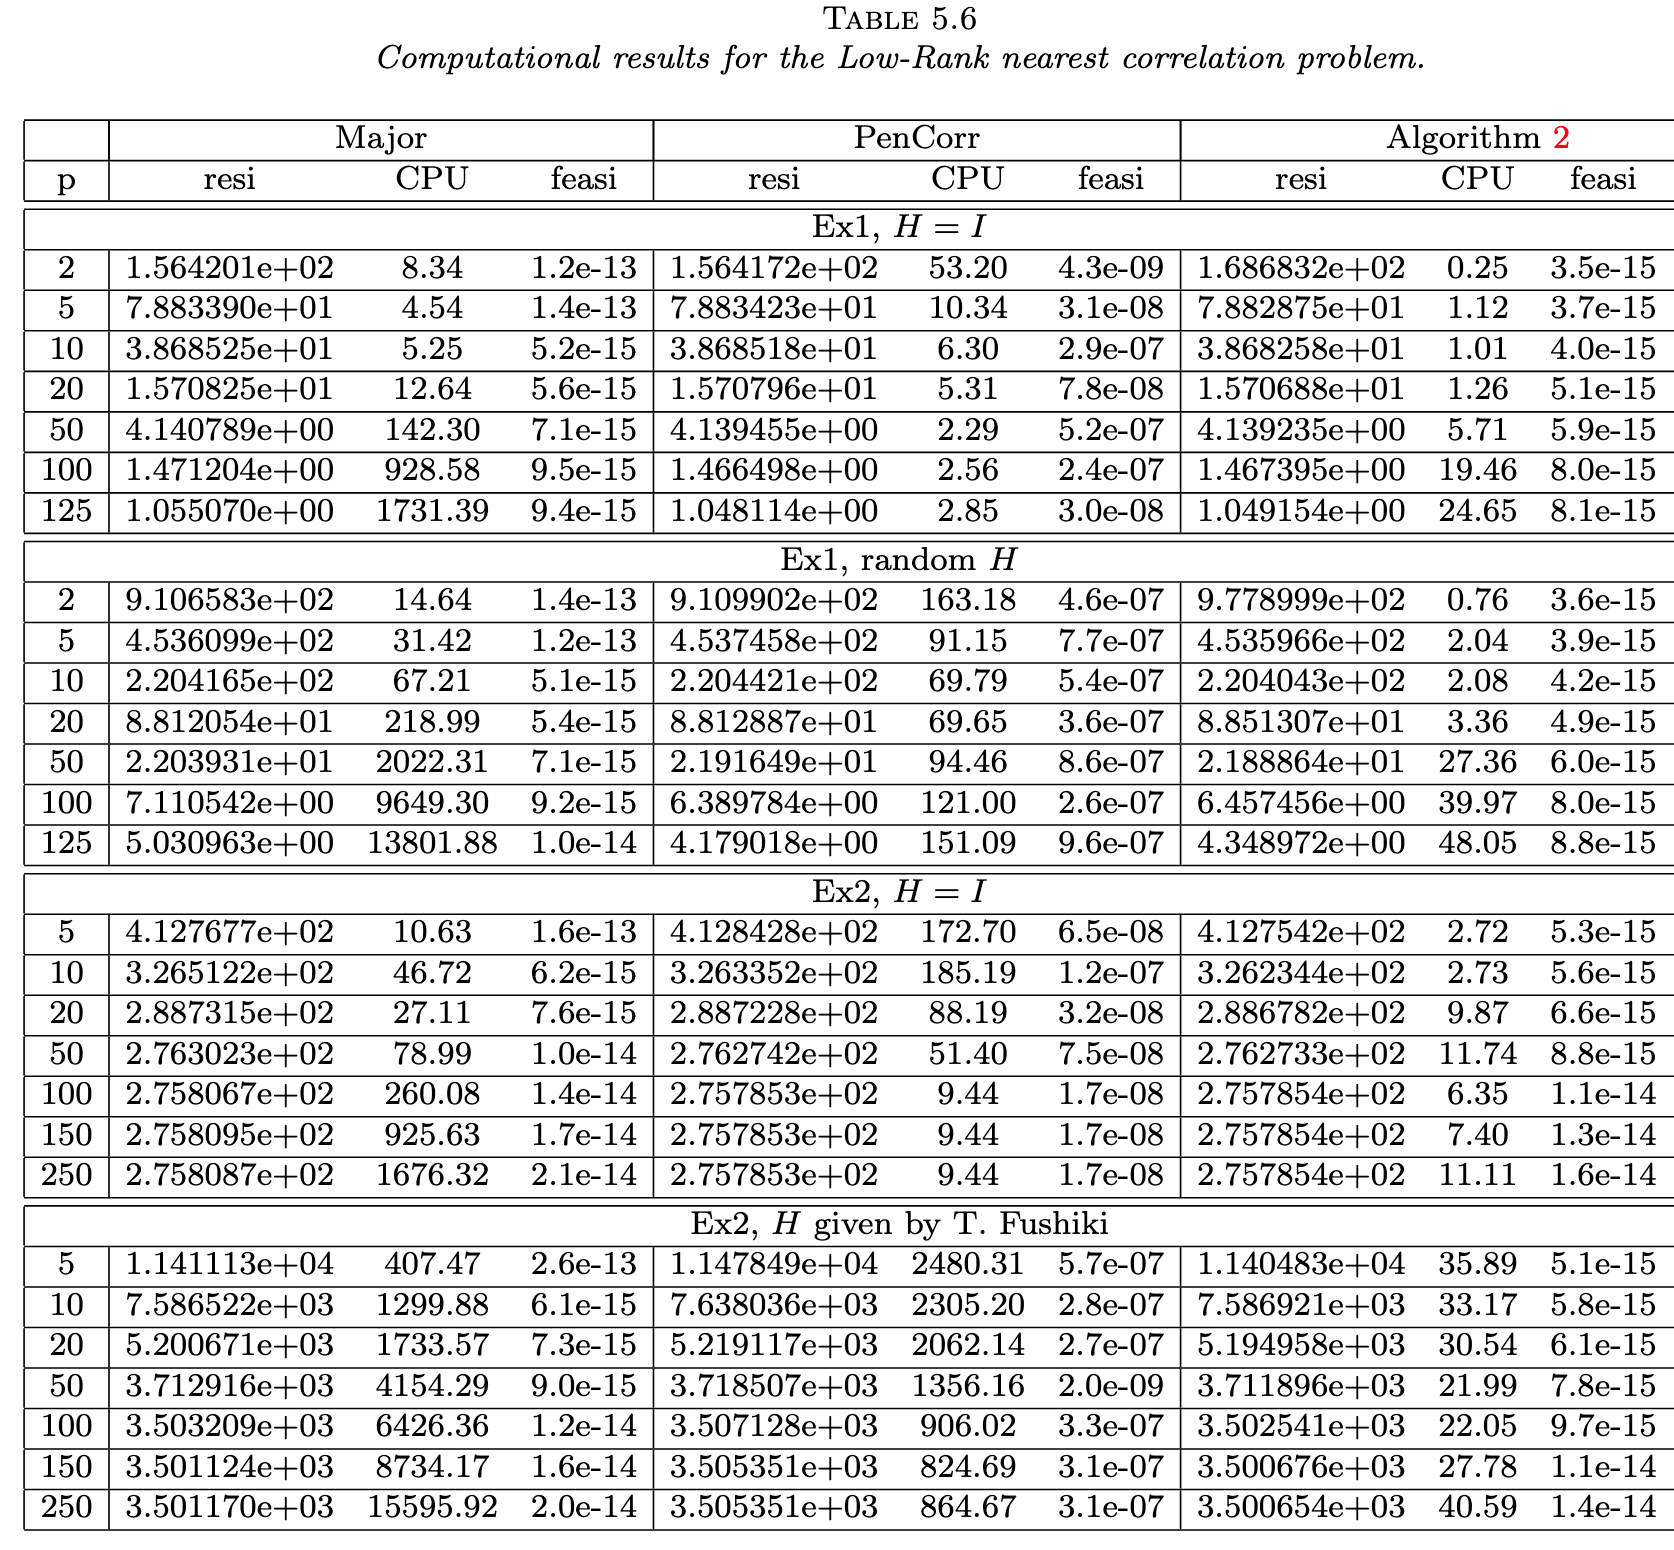
\includegraphics[width=1.0\textwidth]{figures/numerical.png}
                        % \caption{A figure that is next to a certain explanation.}
                \end{figure}
            \end{column}

            \begin{column}{0.35\textwidth}
               \begin{block}{Remarks}
                    \textcolor{red}{"Algorithm 2"} is the proposed method. 
                        \vspace{0.3cm}
                        
                         \textcolor{blue}{resi}: objective value.
                         
                         \textcolor{blue}{CPU}: running time (sec). 
                         
                         \textcolor{blue}{feasi}: infeasibility. 
            
                    \vspace{0.3cm}
                    All 3 metrics are "the lower the better". 

                    \vspace{0.1cm}
                    Improvement is achieved in running time, especially for the nontrivial $H$ cases.\footnote{Thanks to an efficient implementation of the original Cayley transform.}
                    
                \end{block}
            \end{column}
        \end{columns}
    \end{frame}

    \begin{frame}[t]{Codebase repository}
        \vspace{-0.4cm}
        The authors put their MatLab codes -- with quite high-quality implementation -- of this problem to GitHub.\footnote{https://github.com/optsuite/OptM} There are some more extensions, but the usage are similar.  
        $$\min_{X \in \mathbb{R}^{n \times p}} F(X) ~~~~~ \text{subject to   } X^T X = I_p$$ Anyone can use their API in the following way: 

        \begin{figure}
            \centering
                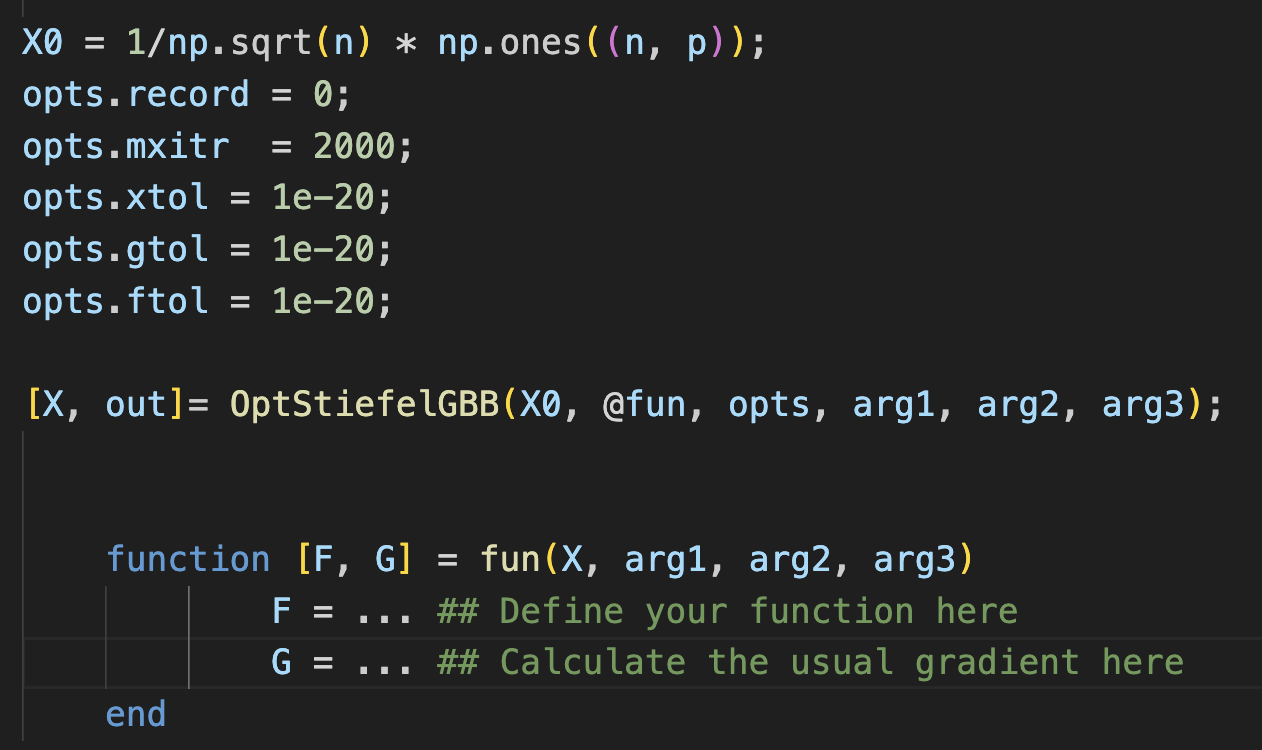
\includegraphics[width=0.7\textwidth]{figures/API.png}
        \end{figure}
        
    \end{frame}



% \begin{frame}[t]{References}
%     \small 
%     M. Vaezi, Z. Ding, and H. V. Poor, Chapter 5 of "Multiple Access Techniques for 5G Wireless Networks and Beyond". Springer Publishing Company, Incorporated, 2018.

%     \vfill 
%     Natasha Devroye, “The interference channel”, \href{http://pfister.ee.duke.edu/nasit16/Devroye_slides.pdf}{online resource (slides)}, 2016

%     \vfill 
%     Abbas El Gamal and Young-Han Kim, “Network Information Theory” Cambridge University Press, USA, 2012.

%     \vfill 
%     L. Xia, Chapter 3, 4 of “On Tightness of Several Achievable Rate Regions in Network Information Theory”, 2016. 

%     \vfill 
%     Peng Xu, Zhiguo Ding, Xuchu Dai and H. Vincent Poor, "NOMA: An Information Theoretic Perspective", arXiv, 2015. 
    
% \end{frame}



%***************************************************************************
%***************************************************************************
\end{document}





































